\newsection{Introduction}

hello hello


% Source - https://tex.stackexchange.com/a/316557
% Posted by Henri Menke
% Retrieved 2026-04-14, License - CC BY-SA 3.0

\begin{figure}[h]
  \centering
  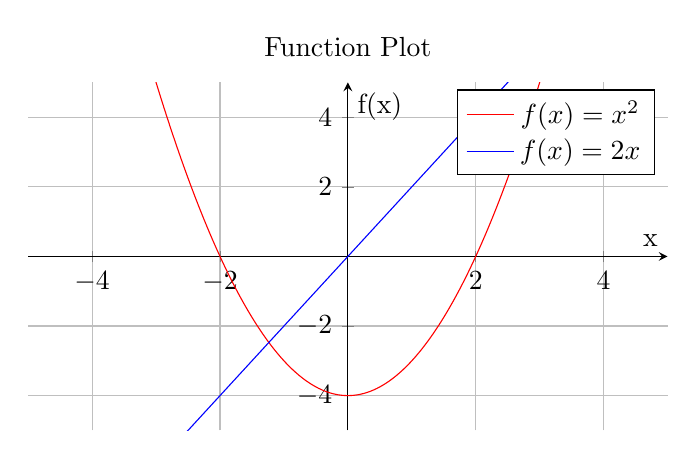
\begin{tikzpicture}
    \begin{axis}[
      title={Function Plot},
      xlabel={x},
      ylabel={f(x)},
      xmin=-5, xmax=5,
      ymin=-5, ymax=5,
      axis lines=middle,
      grid=major,
      width=0.8\textwidth,
      height=6cm,
      trig format plots=deg
    ]
    
    \addplot[
      domain=-5:5,
      samples=100,
      color=red,
      smooth
    ] {x^2-4};
    \addlegendentry{$f(x) = x^2$}

    \addplot[
      domain=-5:5,
      samples=100,
      color=blue,
      smooth
    ] {2*x};
    \addlegendentry{$f(x) = 2x$}
    
    
  \end{axis}
  \end{tikzpicture}
  \caption{Plot of the function x\^2}
  \label{fcn2d:fcn_plot}
\end{figure}
